\documentclass[aps,prl,twocolumn,superscriptaddress,reprint,longbibliography,nofootinbib]{revtex4-2}

\usepackage{graphicx}
\usepackage{dcolumn}
\usepackage{bm}
\usepackage[colorlinks,
citecolor=teal,
linkcolor=teal,
urlcolor=teal]{hyperref}
\usepackage{mathrsfs}
\usepackage{amsfonts,amssymb,amsmath,mathtools}
\usepackage{xcolor}
\usepackage{dsfont}
\usepackage{bbm}
\usepackage{physics}
\usepackage{orcidlink}
\usepackage{amsthm}
\usepackage{tikz}
\usepackage[T1]{fontenc}
\newtheorem{theorem}{Theorem}
\newtheorem{conjecture}{Conjecture}

\newcommand{\rev}[1]{\textcolor{red}{#1}}
\newcommand{\trans}{\mathsf{T}}

% === Custom macros ===
\newcommand{\NL}{\mathrm{GNL}}
\newcommand{\RENYI}{\alpha}
\newcommand{\MNL}{\mathrm{M}_2^{\NL}}

\begin{document}

\title{Non-Local Magic Resources for Fermionic Gaussian States}

\author{Daniele Iannotti\orcidlink{0009-0009-0738-5998}}
\email{d.iannotti@ssmeridionale.it}
\thanks{These two authors contributed equally}
\affiliation{Scuola Superiore Meridionale, Largo S. Marcellino 10, 80138 Napoli, Italy}
\affiliation{INFN Sezione di Napoli, via Cintia, 80126 Napoli, Italy}
\affiliation{ Institut für Theoretische Physik, Universität zu Köln, Zülpicher Strasse 77, 50937 Köln, Germany}

\author{Beatrice Magni\orcidlink{0009-0009-8577-0525}}
\email{bmagni@uni-koeln.de}
\thanks{These two authors contributed equally}
\affiliation{ Institut für Theoretische Physik, Universität zu Köln, Zülpicher Strasse 77, 50937 Köln, Germany}

\author{Riccardo Cioli\orcidlink{0009-0001-1286-3773}}
\email{riccardo.cioli3@unibo.it}
\affiliation{Dipartimento di Fisica e Astronomia, Università di Bologna and INFN, Sezione di Bologna, via Irnerio 46, I-40126 Bologna, Italy}

\author{Alioscia Hamma\orcidlink{0000-0003-0662-719X}}
\email{alioscia.hamma@unina.it }
\affiliation{Scuola Superiore Meridionale, Largo S. Marcellino 10, 80138 Napoli, Italy}
\affiliation{Dipartimento di Fisica `Ettore Pancini', Universit\`a degli Studi di Napoli Federico II, Via Cintia, 80126 Napoli, Italy}
\affiliation{INFN Sezione di Napoli, via Cintia, 80126 Napoli, Italy}

\author{Xhek Turkeshi\orcidlink{0000-0003-1093-3771}}
\email{xturkesh@uni-koeln.de}
\affiliation{ Institut für Theoretische Physik, Universität zu Köln, Zülpicher Strasse 77, 50937 Köln, Germany}

\begin{abstract}
Non-local magic quantifies the nonstabilizerness that local unitaries cannot remove, but its computation requires an intractable optimization. For fermionic Gaussian states and contiguous bipartitions, we prove a closed formula for the R\'enyi-2 non-local stabilizer entropy over local Gaussian unitaries, set by the reduced Majorana covariance matrix. We derive a Page-like curve for random states, logarithmic scaling at the XY critical point, and a quasiparticle picture after quenches. Our result enables measuring fermionic Gaussian-restricted non-local magic via fermionic shadow tomography.
\end{abstract}

\maketitle

\textit{Introduction.}---Entanglement and magic, or nonstabilizerness, are two fundamental notions of quantum complexity that capture complementary aspects of what makes a many-body system genuinely quantum~\cite{Horodecki2009,Chitambar2019resources,Veitch2014resource}.
States with low entanglement admit efficient classical simulation via tensor networks~\cite{Schollw_ck_2011}, whereas states with low magic are accessible to stabilizer-based techniques such as tableau simulation~\cite{Gottesman1998,Bravyi2019simulationofquantum} or Pauli propagation~\cite{dowling2025magic,rudolph2025paulipropagationcomputationalframework}.
While entanglement is a well-characterized concept in many-body physics~\cite{Laflorencie_2016,amico2008entanglement}, the role of magic has only recently come into focus, driven by the development of stabilizer entropies~\cite{Leone2022SRE,leone2024stabilizer}, scalable probes of nonstabilizerness whose computational cost is comparable to that of entanglement entropy~\cite{huang2026fastexactapproachstabilizer,xiao2026exponentiallyacceleratedsamplingpauli,sierant2026computingquantummagicstate} and which have an important operational meaning~\cite{Bittel_2026, Iannotti_2026, cusumano2025nonstabilizernessviolationschshinequalities}.
This advance has stimulated a broad research program, from equilibrium phenomena~\cite{piro2,tarabunga2023manybody,oshino2026stabilizer,hoshino2025stabilizerrenyientropyencodes, aditya2025mpembaeffectsquantumcomplexity} to quantum-circuit and Hamiltonian dynamics~\cite{Turkeshi_2025,odavic2025stabilizer,tirrito2025anticoncentration,falcao2025nonstabilizerness, PhysRevB.106.214316, p8dn-glcw, lio2026quantumstatedesignsmagic, aditya2025growthspreadingquantumresources, Viscardi_2026}.

A central open question concerns the interplay between entanglement and magic~\cite{tirrito2024quantifying,szombathy,Iannotti2025entanglement}.
The recently introduced \emph{non-local magic}~\cite{Cao_2025,qian2025quantumnonlocalnonstabilizerness, munizzi2026magicnoncliffordgatestopological, cao2024non} isolates the irreducible nonstabilizerness that cannot be removed by local basis changes, thereby separating genuinely correlated magic from purely local contributions.
However, non-local magic is defined through a minimization over all local unitaries acting on the full Hilbert space, rendering it intractable beyond a few qubits.
Although estimation schemes exist for matrix-product states~\cite{Cao_2025}, where entanglement remains bounded, which classes of quantum matter admit an analytic characterization of non-local magic, especially in regimes with extensive entanglement, has remained an open question.

In this Letter, we answer this question for fermionic Gaussian states and unitaries. We introduce the fermionic Gaussian-restricted non-local (GNL) magic, and prove (Theorem~\ref{thm:global}) that at R\'enyi index $\RENYI=2$ it admits a closed-form expression in terms of the eigenvalues of the reduced Majorana covariance matrix of a contiguous subsystem of size $\ell$, computable with $\mathrm{poly}(\ell)$ resources.
The key insight is that the minimization over local \emph{Gaussian} unitaries is solved exactly by the BCS canonical form~\cite{BoteroReznik2004}.
This is in stark contrast with the total magic, which requires Majorana Monte Carlo~\cite{Bera_2025} or perfect sampling~\cite{collura2026nonstabilizernessfermionicgaussianstates}, both converging in general with an exponential number of samples.
We leverage this result to obtain an exact Page-like curve for typical fermionic Gaussian states, corroborated by SYK$_2$ eigenstates~\cite{Bera_2025,santra2025complexitytransitionschaoticquantum,jasser2025stabilizer, malvimat2026multipartitenonlocalmagicsyk, njgn-fksh}; logarithmic scaling of non-local magic at the XY critical point via the Fisher--Hartwig approach; a quasiparticle picture~\cite{calabrese2009} for magic spreading after quantum quenches; and diffusive growth in random Gaussian circuits.
Because our result relies solely on two-point correlation functions, it provides a scalable route for the experimental estimation of Gaussian-restricted non-local magic in large-scale quantum processors via fermionic shadow tomography~\cite{Wan_2023}.

\textit{Setup.}---We consider $N$ qubits on a chain $\Lambda=\{1,\dots, N\}$, with Hilbert space dimension $d=2^N$~\cite{Mbeng2024,surace,sierant2026fermionic,sierant2026theorymatchgatecommutant}.
The $2N$ Majorana operators are obtained via the Jordan--Wigner (JW) transformation, $\gamma_{2j-1} = \bigl(\prod_{m<j} Z_m\bigr)X_j$ and $\gamma_{2j} = \bigl(\prod_{m<j} Z_m\bigr)Y_j$, and satisfy $\{\gamma_j,\gamma_k\}=2 \delta_{jk}$.
Fermionic Gaussian unitaries (FGU), or matchgates, act on the Majorana operators as rotations, $U_O\gamma_j U_O^\dagger = \sum_{m}O_{mj}\gamma_m$ with $O\in \mathrm{O}(2N)$; up to the reflection implemented by $X_1=\gamma_1$, they are generated by quadratic Hamiltonians
\begin{equation}
    H= \frac{i}{4}\sum_{m,n=1}^{2N} h_{m,n} \gamma_m\gamma_n\;,\qquad h=-h^{\trans}\;.\label{eq:ham}
\end{equation}
A pure fermionic Gaussian state (FGS) $|\Psi_O\rangle=U_O|\mathbf{0}\rangle$, with $|\mathbf{0}\rangle$ the fermionic vacuum, is fully characterized by its covariance matrix $\Gamma_{mn}=i\langle \Psi_O|[\gamma_m,\gamma_n]|\Psi_O\rangle/2$, given by $\Gamma= O\Gamma_0 O^{\trans}$ with $\Gamma_0=\bigoplus_{m=1}^N \bigl(\begin{smallmatrix}0&-1\\1&0\end{smallmatrix}\bigr)$.

The stabilizer entropy of order $\RENYI$ of a pure state is $M_\RENYI=(1-\RENYI)^{-1}\log_2 \zeta_\RENYI$~\cite{Leone2022SRE}, where $\zeta_\RENYI= d^{-1}\sum_{P\in \mathcal{P}_N} \langle \Psi|P|\Psi\rangle^{2\RENYI}$ is the stabilizer purity and $\mathcal{P}_N$ the set of $N$-qubit Pauli strings; it is a magic monotone for integer $\RENYI\ge 2$~\cite{piro,leone2024stabilizer}.
Throughout, we consider the bipartition $\Lambda = A\sqcup B$ of the chain into the contiguous blocks $A=\{1,\dots,\ell\}$ and $B=\{\ell+1,\dots,N\}$. The non-local magic is~\cite{Cao_2025}
\begin{equation}
    M_\RENYI^\textup{NL}:= \min_{U_A , U_B} M_\RENYI\left[(U_A\otimes U_B)|\Psi\rangle\right]\;,\label{eq:defNLmagic}
\end{equation}
where the minimization is over $\mathrm{U}(2^\ell)\otimes \mathrm{U}(2^{N-\ell})$. This is the magic that cannot be erased by local unitaries; for instance, maximally entangled states have vanishing non-local magic, being locally equivalent to stabilizer states. It is distinct from long-range magic, which cannot be removed by finite-depth local circuits~\cite{Korbany2025}.
The minimization in Eq.~\eqref{eq:defNLmagic} is superexponentially costly; for $\RENYI = 2$, a proxy can be obtained from the Schmidt spectrum~\cite{Cao_2025}.
For fermionic Gaussian states, we introduce the GNL magic
\begin{equation}
    M_\RENYI^\textup{GNL}:= \!\!\min_{U_{O_A} , U_{O_B}} \!\!M_\RENYI\left[(U_{O_A}\otimes U_{O_B})|\Psi\rangle\right],\label{eq:defGNLmagic}
\end{equation}
where the minimization is restricted to the Gaussian unitaries of $A$ and $B$ induced by $O_A\in\mathrm{O}(2\ell)$ and $O_B\in\mathrm{O}(2(N-\ell))$, hence $ M_\RENYI^\textup{NL} \leq  M_\RENYI^\textup{GNL}$. Since $A$ and $B$ are contiguous, $U_{O_A}\otimes U_{O_B}$ is itself a Gaussian unitary of the whole chain, so that Eq.~\eqref{eq:defGNLmagic} amounts to a maximization of $\zeta_2$ over the local orthogonal orbit $\Gamma\mapsto(O_A\oplus O_B)\Gamma(O_A\oplus O_B)^{\trans}$ (End Matter).

\textit{Main result.}---Let $\pm\lambda_i$, with $\lambda_i\in[0,1]$ and $i=1,\dots,\ell$, be the eigenvalues of the $2\ell\times 2\ell$ reduced covariance matrix $i\Gamma_A$ of the Majorana operators of $A$.

\begin{theorem}
\label{thm:global}
For any pure fermionic Gaussian state $|\Psi_O\rangle$ on $N$ modes and the contiguous blocks $A=\{1,\dots,\ell\}$ and $B=\{\ell+1,\dots,N\}$,
\begin{equation}
\begin{split}
    M_{2}^{\mathrm{GNL}}(|\Psi_O\rangle)&=\sum_{i=1}^{\ell}\mathfrak{m}_2(\lambda_i^2)\;,\\
    \mathfrak{m}_2(x)&=-\log_2\!\left(1-x+x^2\right).
\end{split}
    \label{eq:analytic_NL}
\end{equation}
Equivalently, the maximum of the stabilizer purity over the local Gaussian orbit is $\max_{O_A,O_B}\zeta_2=\prod_{i=1}^{\ell}(1-\lambda_i^2+\lambda_i^4)$, attained in the canonical modewise axes of Ref.~\cite{BoteroReznik2004}.
\end{theorem}

Local FGU bring any pure FGS into a canonical modewise form of independent two-mode BCS-like pairs, $\cos\theta_i|00\rangle+\sin\theta_i|11\rangle$, and unpaired modes~\cite{BoteroReznik2004}, a normal form that underlies several descriptions of fermionic Gaussian entanglement~\cite{SpeeSchwaigerGiedkeKraus2018,MorralYepesLangerGammonSmithKrausPollmann2025,langer2026matchgatecircuitrepresentationfermionic}.
We prove that this representative is the \emph{global} maximizer of $\zeta_2$ on the local Gaussian orbit, from which Eq.~\eqref{eq:analytic_NL} follows by a direct computation of the two-qubit stabilizer entropy~\cite{Cao_2025,qian2025quantumnonlocalnonstabilizerness}.
The proof is outlined in the End Matter and given in full in Sec.~S1 of the Supplemental Material (SM)~\cite{SM}. It combines a Wick-theorem representation of $\zeta_2$ as the collision probability of a determinantal point process with two ingredients of independent interest: a sharp bound on the collision probability of a Slater determinant in terms of its transpose overlap, and a determinant inequality for positive matrices of rank at most two.

For integer $\RENYI>2$, we conjecture that the same structure survives,
\begin{equation}
\begin{split}
      M_{\RENYI}^{\mathrm{GNL}} &= \sum_{i=1}^{\ell}\mathfrak{m}_\RENYI(\lambda_i^2)\;,\\
      \mathfrak{m}_\RENYI(x)&=\frac{1}{1-\RENYI}\log_2\! \frac{\left(1-x \right)^{\RENYI }\!+1+ x^{ \RENYI }}{2}\;,
\end{split}
    \label{eq:analytic_NL_alpha}
\end{equation}
which reduces to Eq.~\eqref{eq:analytic_NL} at $\RENYI=2$. This conjecture is supported by extensive variational optimization (SM, Sec.~S2) and reproduces the same phenomenology as the $\RENYI=2$ case (SM, Sec.~S4); below we focus on $\RENYI=2$.

Several remarks are in order. First, for $\ell\le 2$ the Gaussian minimization coincides with the full one, $M_2^{\mathrm{NL}}=M_2^{\mathrm{GNL}}$, and Eq.~\eqref{eq:analytic_NL} reproduces the expression of Ref.~\cite{Cao_2025}; for larger subsystems, non-Gaussian local unitaries can further decrease the magic, so that Theorem~\ref{thm:global} provides an upper bound, $M_2^{\mathrm{NL}}\le M_2^{\mathrm{GNL}}$.
Second, Eq.~\eqref{eq:analytic_NL} requires only $\mathrm{poly}(\ell)$ operations, whereas even the total stabilizer entropy of FGS requires in the worst case an exponential number of samples~\cite{Bera_2025,collura2026nonstabilizernessfermionicgaussianstates}.
Third, entanglement is necessary but not sufficient for non-local magic: $\mathfrak{m}_2(\lambda^2)$ vanishes both for unentangled ($\lambda=1$) and for maximally entangled ($\lambda=0$) modes. For instance, the rainbow state $\bigotimes_{j=1}^{N/2} (|0_j 0_{N+1-j}\rangle + |1_j 1_{N+1-j}\rangle)/\sqrt2$ is a FGS with maximal entanglement across $A=\{1,\dots,N/2\}$, i.e., $\lambda_j=0$, yet it is a stabilizer state with $M_2^{\mathrm{NL}}=M_2^{\mathrm{GNL}}=0$. Local non-Clifford rotations only add local magic; genuine non-local magic requires modes at intermediate entanglement, $0<\lambda_j<1$, e.g., generated by a joint non-Clifford Gaussian rotation of each pair~\cite{huang2026dismagickerunitarygatenonstabilizerness}.
Finally, since Eq.~\eqref{eq:analytic_NL} depends only on $\Gamma_A$, a polynomial number of two-point functions, GNL magic is accessible via fermionic shadow tomography~\cite{Wan_2023}: random matchgate circuits followed by computational-basis measurements reconstruct $\Gamma_A$ with accuracy $\epsilon_\Gamma$ and failure probability $\delta$ with $O(\ell^2\log(\ell/\delta)/\epsilon_\Gamma^2)$ shots; the propagation of this error to $M_2^{\mathrm{GNL}}$ is discussed in the SM, Sec.~S3. This opens a scalable route beyond the recent two-qubit demonstration of non-local magic~\cite{ahmad2025experimentaldemonstrationnonlocalmagic}.

\textit{Typical states.}---We first consider states $|\Psi_O\rangle$ with Haar-random $O\in \mathrm{O}(2N)$, whose statistics is invariant under mode permutations, and $A=\{1,\dots,\ell\}$, $\ell\le N/2$.
The variables $x_m=\lambda_m^2$ form a Jacobi ensemble~\cite{Mehta2004,PhysRevB.103.L241118} with joint distribution $\propto\prod_{i<j}(x_i-x_j)^2\prod_m x_m^{-1/2}(1-x_m)^{N-2\ell}$.
Since $M_2^\mathrm{GNL}$ is a sum of single-mode terms, its quenched average $\overline{M}_2^\mathrm{GNL}\equiv \mathbb{E}_{O}[M_2^\mathrm{GNL}]=\int_0^1 \mathfrak{m}_2(x)\varrho^{(\ell)}(x)dx$ only requires the one-point density $\varrho^{(\ell)}(x)$, which is known exactly at finite $N$ (End Matter). In the thermodynamic limit $\ell,N\to\infty$ at fixed $r=\ell/N\in[0,1/2]$, $\varrho^{(\ell)}/N$ converges to the free Jacobi law $\varrho_r(x) = \sqrt{(c-x)x}/[2\pi x(1-x)]$ supported on $[0,c]$, with $c=4r(1-r)$. Setting $x=c\sin^2\theta$, the GNL magic density $\overline{\mathsf{m}}_2^\mathrm{GNL}:=\overline{M}_2^\mathrm{GNL}/N$ reads
\begin{equation}
\overline{\mathsf{m}}_2^\mathrm{GNL}(r)\simeq \frac{c}{\pi}\int_0^{\pi/2} \frac{\cos^2 \theta}{1-c\sin^2\theta}\, \mathfrak{m}_2(c\sin^2 \theta)\,d\theta\;,\label{eq:ziopin2}
\end{equation}
symmetric under $r\to 1-r$.
At half partition, $\overline{\mathsf{m}}_2^\mathrm{GNL}(1/2)= 2-\log_2(2+\sqrt{3})$, while for $r\to0$ we find $\overline{\mathsf{m}}_2^\mathrm{GNL}\simeq r^2/\ln 2$.
This \emph{GNL magic Page curve} [Fig.~\ref{fig:typicality}(a)] has a quadratic onset for every $\RENYI$ (SM, Sec.~S4), with a transparent origin: when $\ell=O(1)$ and $N\to\infty$, the modes of $A$ are almost maximally entangled and carry no non-local magic. This is in sharp contrast with the entanglement Page curve, which grows linearly for small $r$~\cite{PhysRevE.106.034118,PhysRevLett.125.180604,PhysRevB.103.L241118}.

To test universality beyond Haar-random states, we consider mid-spectrum eigenstates of the SYK$_2$ model, Eq.~\eqref{eq:ham} with $h_{m,n}\sim \mathcal{N}(0,1/N)$, obtained by flipping a random subset of $N/4$ to $N/2$ single-particle modes in the ground state (SM, Sec.~S5). Averaging over $10^3$ disorder realizations and $200$ eigenstates each, the data converge to Eq.~\eqref{eq:ziopin2} as $N$ increases [Fig.~\ref{fig:typicality}(b)].

\begin{figure}[t!]
    \centering
    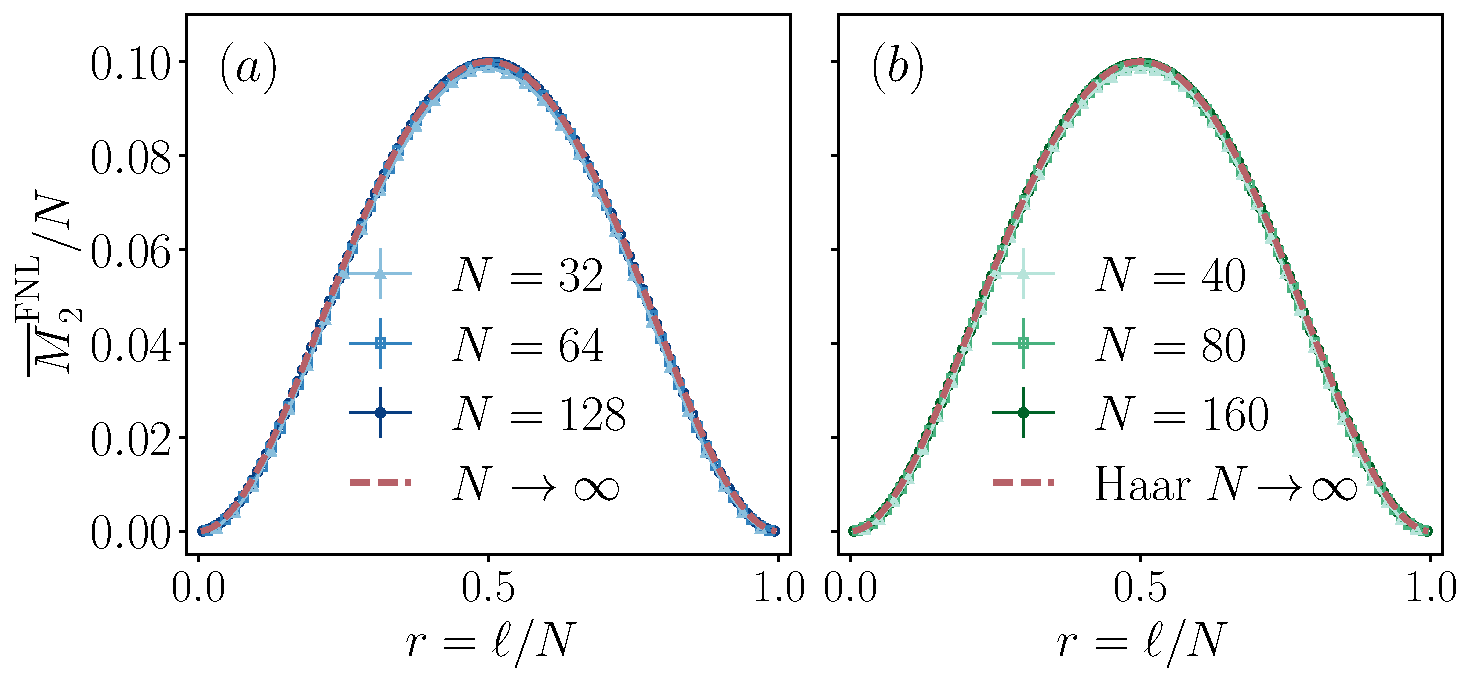
\includegraphics[width=\columnwidth]{fig1_typicality.pdf}
    \caption{\textbf{GNL magic of typical fermionic Gaussian states.}
    (a)~Page curve for Haar-random FGS: $\overline{M}_2^{\mathrm{GNL}}/N$ vs $r=\ell/N$, compared with the $N\to\infty$ prediction, Eq.~\eqref{eq:ziopin2}.
    (b)~Average GNL magic of SYK$_2$ mid-spectrum eigenstates, in quantitative agreement with Eq.~\eqref{eq:ziopin2}.}
    \label{fig:typicality}
\end{figure}

\begin{figure*}[t!]
    \centering
    \begin{tikzpicture}
    \node[anchor=south west,inner sep=0] (img) at (0,0) {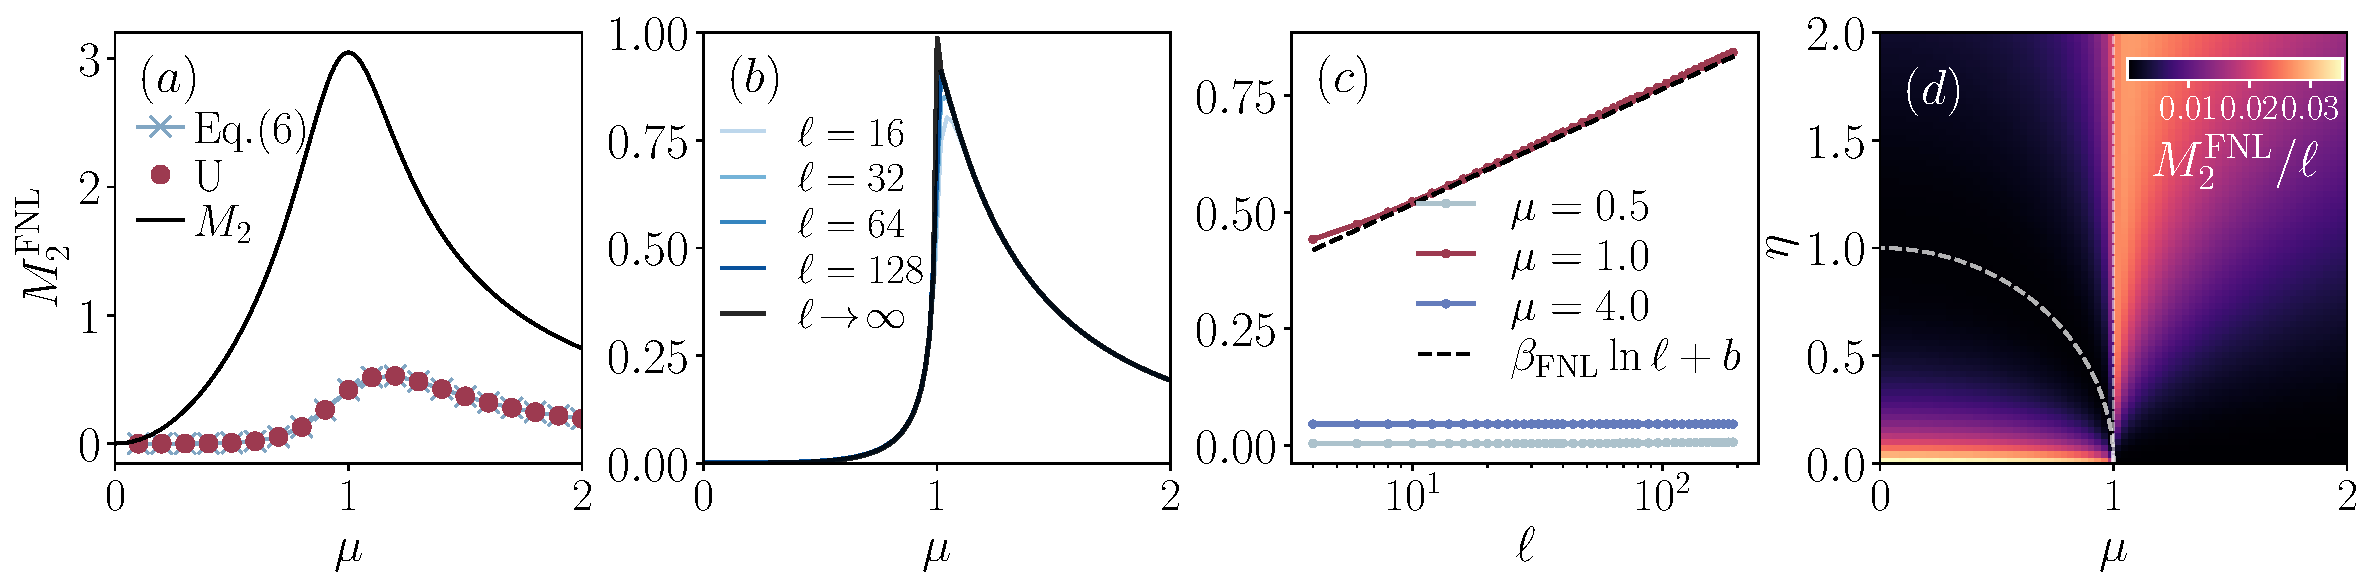
\includegraphics[width=\linewidth]{fig1_equilibrium.pdf}};
    \begin{scope}[x={(img.south east)},y={(img.north west)}]
    \fill[white] (0.0795,0.735) rectangle (0.131,0.825);
    \node[anchor=west,inner sep=0,font=\fontsize{10}{10}\selectfont] at (0.0805,0.778) {Eq.(\ref*{eq:analytic_NL})};
    \end{scope}
    \end{tikzpicture}
    \caption{%
    \textbf{Equilibrium GNL magic in the Ising and XY chains.}
    (a)~Ising ground state with $N=8$, $\ell=4$: Eq.~\eqref{eq:analytic_NL} (crosses) agrees with the brute-force minimization over all local unitaries $U_A \otimes U_B$ (red markers) to numerical precision; the black line is the total stabilizer entropy $M_2$.
    (b)~$M_2^{\mathrm{GNL}}$ vs transverse field $\mu$ in the thermodynamic limit for $\ell = 16, 32, 64, 128$; the black curve is the exact $\ell \to \infty$ result, Eq.~\eqref{eq:NL_peschel2}. The GNL magic peaks at the critical point $\mu_c = 1$.
    (c)~$M_2^{\mathrm{GNL}}(\ell)$ at criticality ($\mu = 1$, red) grows logarithmically: the dashed line is the fit $\beta_{\mathrm{fit}}\ln\ell+b$, with $\beta_{\mathrm{fit}} \approx 0.1072$ and $b \approx 0.27$, in agreement with Eq.~\eqref{eq:alpha_NL}. In the gapped phases ($\mu = 0.5$, $4.0$), $M_2^{\mathrm{GNL}}$ saturates.
    (d)~$M_2^{\mathrm{GNL}}/\ell$ over the XY phase diagram ($\mu$, $\eta$), from the exact corner-transfer-matrix formula: the GNL magic concentrates near the critical lines.
    }
    \label{fig:Ising_model}
\end{figure*}

\textit{Ground states.}---We now consider the XY chain with periodic boundary conditions,
\begin{equation}
    H = -\sum_{j=1}^{N}\!\left[\frac{1+\eta}{2}X_j X_{j+1} + \frac{1-\eta}{2}Y_j Y_{j+1} + \mu Z_j\right],
    \label{eq:xy}
\end{equation}
which the JW transformation maps onto a quadratic Majorana chain of the form of Eq.~\eqref{eq:ham}.
We study it as a \emph{fermionic} model: its ground state is a FGS and the natural notion of locality is that of the fermionic modes, so that $M_2^{\mathrm{GNL}}$ is the non-local magic of the free-fermion problem, and we take the contiguous block $A=\{1,\dots,\ell\}$.
For $N\to\infty$ at fixed $\ell$, $\Gamma_A$ is a block-Toeplitz matrix with a $2\times2$ symbol $g(k)$ fixed by the Bogoliubov angle $\theta_k$ (End Matter). Hence, $M_2^{\mathrm{GNL}}$ is computed at cost $O(\ell^3)$, and its asymptotics for $\ell\gg1$ is controlled by the strong Szeg\H{o} theorem for smooth symbols and by the Fisher--Hartwig formula for singular ones~\cite{Jin_2004,Its_2005}.
Since $|\det g(k)| = 1$, volume-law scaling is excluded; in the gapped phases, where $\theta_k$ is analytic, $M_2^{\mathrm{GNL}}$ saturates with exponentially small corrections~\cite{simon2010szego}, while logarithmic growth can only arise from singularities of the symbol, as at the Ising critical point $\mu=1$, $\eta=1$.

Off criticality, the single-particle entanglement energies of a semi-infinite cut are known from corner transfer matrices~\cite{Peschel2009,Eisler2017}: they are equally spaced, $\varepsilon_n^{\mathrm{ent}} = (2n+1)\varepsilon$ for $\mu>1$ and $\varepsilon_n^{\mathrm{ent}} = 2n\varepsilon$ for $\mu<1$, with $n=0,1,\dots$ and $\varepsilon$ given in the End Matter. Since $\lambda_n = \tanh(\varepsilon_n^{\mathrm{ent}}/2)$~\cite{Peschel2004}, and the block has two boundaries,
\begin{equation}
    M_2^{\mathrm{GNL}}(\ell) \simeq 2\sum_{n=0}^{\infty} \mathfrak{m}_2\!\left[\tanh^2\left(\varepsilon_n^{\mathrm{ent}}/2\right)\right],
    \label{eq:NL_peschel2}
\end{equation}
up to corrections exponentially small in $\ell/\xi$, with $\xi$ the correlation length. As $\mathfrak{m}_2(x)\simeq(1-x)/\ln 2$ for $x \to 1$, the series converges rapidly.
In the ordered phase of the Ising chain ($\eta=1$, $\mu<1$), the GNL magic is strongly suppressed: the $n=0$ mode is maximally entangled ($\lambda_0=0$), while all other modes are exponentially close to unentangled ($\lambda_n\to1$), so that every mode contributes an exponentially small amount, vanishing exactly in the GHZ limit $\mu\to0$. This is a striking example of a phase with area-law entanglement but negligible non-local magic.

At $\mu=1$, the gap closes, $\varepsilon\to0$, the series in Eq.~\eqref{eq:NL_peschel2} diverges, and $\theta_k$ develops a jump at $k=0$. The Fisher--Hartwig asymptotic density of the eigenvalues $\lambda\in[0,1)$ for a block with two boundaries, $\rho(\lambda) \simeq 2\ln\ell\,[\pi^2(1-\lambda^2)]^{-1}$~\cite{Its_2005}, yields $M_2^{\mathrm{GNL}}(\ell)\simeq \beta_{\mathrm{GNL}}\ln\ell$, with
\begin{equation}
    \beta_{\mathrm{GNL}} = \frac{2}{\pi^2}\int_{0}^{1} \frac{\mathfrak{m}_2(\lambda^2)}{1-\lambda^2}\, d\lambda= \frac{\pi ^2-\ln ^2\left(7-4 \sqrt{3}\right)}{\pi ^2 \ln 16}\;,
    \label{eq:alpha_NL}
\end{equation}
the non-local magic analog of $S \simeq (c/3)\ln\ell$~\cite{Calabrese2004entanglement}, with the central charge $c$ replaced by $\beta_{\mathrm{GNL}}$.

Figure~\ref{fig:Ising_model} benchmarks these predictions. In panel (a), Eq.~\eqref{eq:analytic_NL} agrees with a brute-force minimization over the full group $\mathrm{U}(2^\ell)\otimes\mathrm{U}(2^{N-\ell})$ for $N=8$, $\ell=4$. For a general model, however, we do not expect such agreement, and only $M_2^{\mathrm{NL}}\le M_2^{\mathrm{GNL}}$ is expected to hold (SM, Sec.~S2); nevertheless, throughout the XY phase diagram and for the sizes accessible to exact minimization, we find that the agreement persists~\cite{zenodo}. In panel (b), exact numerics for $N=10^6$ agree with Eq.~\eqref{eq:NL_peschel2}. In panel (c), a fit for $\ell > 50$ at $\mu = 1$ gives $\beta_{\mathrm{fit}} \approx 0.1072$, in excellent agreement with Eq.~\eqref{eq:alpha_NL}. Panel (d) shows that over the full XY phase diagram the GNL magic is concentrated near the critical lines.

These results reflect an area law. Since $\mathfrak{m}_2(\lambda^2)\le 2\,\mathfrak{f}[(1+\lambda)/2]$, with $\mathfrak{f}$ the binary entropy, Eq.~\eqref{eq:analytic_NL} implies $M_2^{\mathrm{GNL}}\le 2S(A)$, the Gaussian analog of the bound of Ref.~\cite{Cao_2025}; by Hastings' theorem~\cite{Hastings_2007}, $M_2^{\mathrm{NL}}\le M_2^{\mathrm{GNL}}\le 2C_{\mathrm{ent}}|\partial A|$ in unique gapped ground states of one-dimensional local free-fermion Hamiltonians (End Matter).

\begin{figure*}[t!]
    \centering
    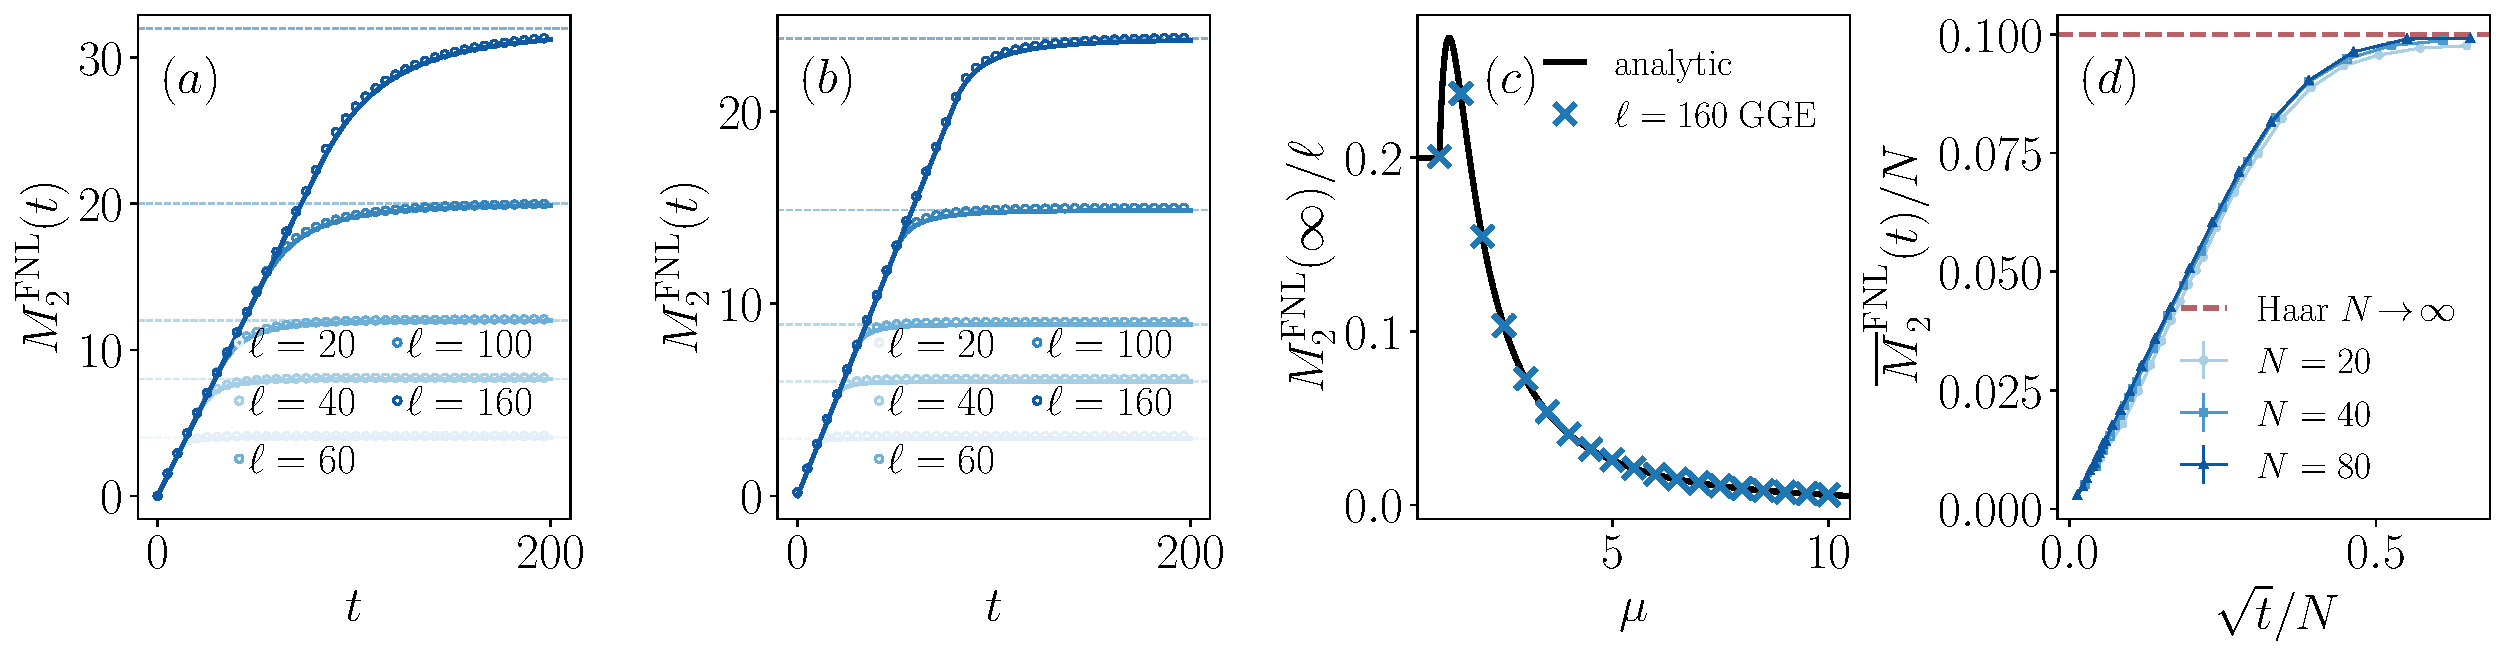
\includegraphics[width=\linewidth]{fig2_dynamics_4panel.pdf}
    \caption{%
    \textbf{Dynamics of GNL magic.}
    (a)~Quench at $\eta=1$ from the fully polarized state ($\mu_0\to\infty$) to the critical point ($\mu=1$): exact numerics (circles) agree with the quasiparticle prediction, Eq.~\eqref{eq:fagotti_mnl} (solid lines), for $\ell = 20, 40, 60, 100, 160$. Dashed lines mark the stationary value, Eq.~\eqref{eq:mnl_stationary}.
    (b)~Same for the quench $\mu_0 = 2 \to \mu = 1$, showing weaker GNL magic production due to the smaller Bogoliubov mismatch.
    (c)~Stationary density $M_2^{\mathrm{GNL}}(\infty)/\ell$ vs the post-quench field $\mu$ ($\mu_0\to\infty$): Eq.~\eqref{eq:mnl_stationary} (solid) and GGE numerics at $\ell = 160$ (crosses).
    (d)~Random Gaussian circuits: $\overline{M}_2^{\mathrm{GNL}}/N$ vs $\sqrt{t}/N$ for $N = 20, 40, 80$, showing diffusive growth and saturation to the Haar value $\overline{\mathsf{m}}_{2}^{\mathrm{GNL}}(1/2)=2-\log_2(2+\sqrt{3})$ (dashed line).}
    \label{fig:dynamics}
\end{figure*}

\textit{Quench dynamics.}---We now turn to quantum quenches in the Ising chain ($\eta=1$): the system is prepared in the ground state of $H(\mu_0)$ and evolved with $H(\mu)$, $\mu\neq\mu_0$.
The state remains Gaussian, and $\Gamma_A(t)$ is block-Toeplitz with a time-dependent symbol fixed by the post-quench dispersion $\varepsilon_k$ and by the mismatch $\Delta\theta_k = \theta_k - \theta_k^{(0)}$ between post- and pre-quench Bogoliubov angles (End Matter)~\cite{Calabrese2005evolution}.
At long times, dephasing leads to a generalized Gibbs ensemble (GGE)~\cite{Calabrese2005evolution,vidmar2017entanglement} with stationary eigenvalues $\lambda_k^\infty=|\cos\Delta\theta_k|$, and the Szeg\H{o} theorem gives
\begin{equation}
    M_2^{\mathrm{GNL}}(\infty) = \frac{\ell}{\pi}\int_0^\pi\! dk\; \mathfrak{m}_2\!\left(\sin^2\!\Delta\theta_k\right)\;,
    \label{eq:mnl_stationary}
\end{equation}
i.e., the quench generically produces volume-law GNL magic.
Equation~\eqref{eq:mnl_stationary} closely parallels the entanglement entropy of the same quench~\cite{Calabrese2005evolution}, $S=(\ell/\pi) \int_0^\pi dk\, \mathfrak{f}\bigl(\sin^2(\Delta\theta_k/2)\bigr)$: in terms of $\lambda_k^{\infty}$, the entanglement weight $\mathfrak{f}[(1+\lambda_k^{\infty})/2]$ is replaced by the magic weight $\mathfrak{m}_2[(\lambda_k^{\infty})^2]=\mathfrak{m}_2(\sin^2\!\Delta\theta_k)$, where we used $\mathfrak{m}_2(x)=\mathfrak{m}_2(1-x)$.
This parallel extends to all times. Writing $M_2^{\mathrm{GNL}}$ as a contour integral of $\frac{d}{d\lambda}\ln\det(\lambda-i\Gamma_A)$ and evaluating the moments $\mathrm{Tr}(i\Gamma_A)^{2n}$ via the multidimensional stationary-phase approach of Ref.~\cite{Fagotti2008} (End Matter), we derive the quasiparticle formula
\begin{equation}
    M_2^{\mathrm{GNL}}(\ell,t) \simeq \int_0^\pi\!\frac{dk}{\pi}\,\min\!\bigl(2|v_k|\,t,\;\ell\bigr)\;\mathfrak{m}_2\!\bigl(\sin^2\Delta\theta_k\bigr),
    \label{eq:fagotti_mnl}
\end{equation}
valid for $\ell, t \gg 1$ at fixed $t/\ell$, with $v_k = d\varepsilon_k/dk$ the group velocity.
Equation~\eqref{eq:fagotti_mnl} predicts linear growth up to $t^* = \ell/(2v_{\max})$, followed by saturation to Eq.~\eqref{eq:mnl_stationary}, and has a transparent interpretation~\cite{Calabrese2005evolution,Fagotti2008}: the quench creates pairs of entangled quasiparticles that propagate ballistically with velocities $\pm v_k$, and a pair contributes to the GNL magic of $A$ only when one partner is inside $A$ and the other outside. The magic carried by each pair, $\mathfrak{m}_2(\sin^2\Delta\theta_k)$, vanishes both when $\Delta\theta_k = 0$ (no entanglement production) and when $\Delta\theta_k = \pi/2$ (maximally entangled but stabilizer-like pairs), and is maximal in between.
Figures~\ref{fig:dynamics}(a)--(c) show excellent agreement between Eqs.~\eqref{eq:mnl_stationary} and~\eqref{eq:fagotti_mnl} and exact numerics, obtained by diagonalizing $\Gamma_A(t)$, for the quenches $\mu_0 = \infty \to 1$ and $\mu_0 = 2 \to 1$ [panels (a), (b)] and for $\mu_0\to\infty$ at varying $\mu$ [panel (c)].

Finally, we consider brickwork circuits of nearest-neighbor Gaussian gates, each drawn from the Haar measure on $\mathrm{SO}(4)$, acting on $|\mathbf{0}\rangle$, with the half-chain bipartition $A=\{1,\dots,N/2\}$~\cite{tirrito2025magicphasetransitionsmonitored} (SM, Sec.~S5).
In contrast with the ballistic spreading of integrable quenches, operator spreading in such circuits is diffusive~\cite{dias2021diffusiveoperatorspreadingrandom,swann}. At early times the modes of $A$ are nearly unentangled, and $\mathfrak{m}_2(x) \simeq (1-x)/\ln 2$ for $x\to1$ gives $M_2^{\mathrm{GNL}}(t) \simeq [2\ell-\mathrm{Tr}(i\Gamma_A(t))^2]/(2\ln 2)=\|\Gamma_{AB}(t)\|_{\mathrm{HS}}^2/(2\ln 2)$, with $\Gamma_{AB}$ the off-diagonal block of $\Gamma$, governed by the diffusive spreading of two-point correlations across the cut~\cite{dias2021diffusiveoperatorspreadingrandom}, so that $M_2^{\mathrm{GNL}} \propto \sqrt{t}$ for $1 \ll t \ll N^2$.
Figure~\ref{fig:dynamics}(d) shows an excellent data collapse of $\overline{M}_2^{\mathrm{GNL}}(t)/N$ as a function of $\sqrt{t}/N$, interpolating between $\sqrt{t}$ growth and saturation at the Page value $\overline{\mathsf{m}}_{2}^{\mathrm{GNL}}(1/2)$ on the diffusive timescale $t\sim N^2$.

\textit{Conclusions.}---We have proved an exact closed form for the fermionic Gaussian-restricted non-local magic of Gaussian states at $\RENYI=2$ for contiguous bipartitions, and conjectured its extension to $\RENYI>2$. By reducing the minimization over local Gaussian unitaries to a single diagonalization of the reduced covariance matrix, it establishes fermionic Gaussian states as a broad class of highly entangled many-body systems where Gaussian-restricted non-local magic is exactly tractable, and provides an upper bound on the unrestricted one. We used it to derive an exact Page-like curve, logarithmic scaling at criticality, a quasiparticle picture after quenches and diffusive growth in random circuits.
This tractability opens several directions: fermionic Gaussian states in higher dimensions, where entanglement is sensitive to the Fermi surface~\cite{swingle2010entanglement}; whether $\beta_{\mathrm{GNL}}$ captures universal features of the underlying conformal field theory~\cite{Calabrese2004entanglement}, and the extension to interacting integrable models~\cite{Alba_2017,alba2019,Kudler_Flam_2021}; disordered~\cite{evers,sierant2020,IGLOI_2005,Monthus_2018,ruggiero2022} and topological~\cite{Kitaev2001chain,Kitaev_2006,beri,gskb-t5ql} systems; symmetry-resolved non-local magic~\cite{Goldstein,Bianchi_2022,aditya2026coherencedynamicsquantummanybody,iannotti2026nonstabilizernessu1symmetrychaotic, cepollaro2025stabilizerentropysubspaces, Esposito_2024} and quantum Mpemba effects~\cite{Ares_2023,Ares_2025,aditya2025mpembaeffectsquantumcomplexity}; and monitored~\cite{FisherRandom2023,Li_2025,oshima} and non-Hermitian~\cite{Ashida_2020,kawabata2026nonhermitiandisorderedsystems,schirooooo,gallo,granet,lapierre2025entanglementtransitionsstructuredrandom} free-fermion dynamics, where our formula applies along each quantum trajectory.

\textit{Note added.}---While preparing this manuscript, we became aware of a closely related independent work by M. Collura, B. Beri, and E. Tirrito~\cite{collura2026nonlocalnonstabilizernessfreefermion}. When overlapping, our results are consistent.

\begin{acknowledgments}
This work is dedicated to Ada. We are particularly indebted to P. Sierant for spotting a mistake in a prior version of this manuscript, and we thank the anonymous referees for their careful reading and, in particular, for pointing out the role of the contiguity of the bipartition in Theorem~\ref{thm:global}, the misprint in the Jacobi weight, and a simpler proof of a lemma in the SM.
We thank L. Leone, A. Russotto, P. Calabrese, L. Piroli, and J. Odavi\'c for comments and collaborations on related topics.
D.I. and B.M. acknowledge the Les Houches Summer School 2025 on Exact Solvability and Quantum Information, which facilitated work on this subject.
D.I. acknowledges support from COST Action THEORY-CHALLENGES CA22113 under Short-Term Scientific Mission (STSM) grant E-COST-GRANT-CA22113-6901e967 and Research Grants in Germany, 2026 (57812126) from the German Academic Exchange Service (DAAD).
B.M. and X.T. acknowledge support from DFG Emmy Noether Programme proposal "Digital Quantum Matter Out-of-Equilibrium" No. 560726973, DFG under Germany's Excellence Strategy – Cluster of Excellence Matter and Light for Quantum Computing (ML4Q) EXC 2004/2 – 390534769, and DFG Collaborative Research Center (CRC) 183 Project No. 277101999 - project B01.
A.H. acknowledges support from PNRR MUR project PE0000023-NQSTI and the PNRR MUR project CN00000013-ICSC.
% TODO (authors): confirm or edit the following AI-use statement before submission.
\rev{Generative AI tools were used to assist in the preparation and editing of parts of this manuscript and of the Supplemental Material. All derivations and numerical results were checked by the authors, who take full responsibility for the content.}
\end{acknowledgments}

\textit{Data availability.}---The data generated in this study will be made publicly available on Zenodo upon publication.

\nocite{Bapat1989,HornJohnson2012,Hough2006,MR38136,bhatia2013matrix,sfeo}
\bibliography{ref_current}

\section*{End Matter}

\appendix

\section{Contiguous blocks and strategy of the proof of Theorem~\ref{thm:global}}
\label{em:proof}

\textit{Local Gaussian orbit.}---For the blocks $A=\{1,\dots,\ell\}$ and $B=\{\ell+1,\dots,N\}$ of Theorem~\ref{thm:global}, $T_{\pi_{AB}}$ is the identity. The JW strings of the Majorana operators of $A$ do not leave $A$, and those of $B$ differ from the ones defined within $B$ only by the parity $P_A=\prod_{m\in A}Z_m$ of $A$. Since $U_{O_A}P_AU_{O_A}^\dagger=\det(O_A)P_A$, the qubit unitary $U_{O_A}\otimes U_{O_B}$ acts on the Majorana operators of the chain as $O_A\oplus\det(O_A)\,O_B$, i.e., it coincides up to a phase with a Gaussian unitary of the chain in $\mathrm{O}(2\ell)\oplus\mathrm{O}(2(N-\ell))$. As $(O_A,O_B)\mapsto(O_A,\det(O_A)\,O_B)$ is a bijection, Eq.~\eqref{eq:defGNLmagic} amounts to maximizing $\zeta_2$ over the orbit $\Gamma\mapsto(O_A\oplus O_B)\Gamma(O_A\oplus O_B)^{\trans}$.
This is where contiguity enters: for non-contiguous bipartitions, the qubits of $A$ must be brought together by a permutation that does not preserve the Gaussian structure, and the identification fails.

\textit{Strategy of the proof.}---On the local Gaussian orbit, $\zeta_2$ is the collision probability of a determinantal distribution which depends on two independent rotations and on \emph{all} minors of the matrix parametrizing the state, so that it is not evidently maximized at the canonical point. The proof (SM, Sec.~S1) is a chain of steps, each of which either removes one of these complications exactly, or bounds the functional by a simpler one that is tight at the canonical point.
(1)~Wick's theorem turns $\zeta_2$ into the collision probability $d\sum_S p_S^2$ of the projection determinantal point process with kernel $K=(\mathbb{I}+i\Gamma)/2$~\cite{collura2026nonstabilizernessfermionicgaussianstates}.
(2)~For any isometry $Q\in\mathbb{C}^{n\times k}$, the collision probability of the associated Slater determinant obeys $\mathcal{C}(Q)\le 2^{-k}\det(\mathbb{I}+\Sigma^\dagger\Sigma)$, with $\Sigma=Q^{\trans}Q$ the transpose overlap; this sharp bound is proved by induction on $n$.
(3)~In the BCS parametrization, the dependence on the local rotations is packaged into $Z=O_AZ_0O_B^{\trans}$, with $Z_0=\bigoplus_j(\mathbb{I}_2+i\lambda_jJ)/\sqrt{1-\lambda_j^2}$ and $J=\bigl(\begin{smallmatrix}0&1\\-1&0\end{smallmatrix}\bigr)$, and $\zeta_2$ becomes, up to an orbit-invariant constant, the sum $\mathsf{F}(Z)=\sum_{|I|=|J|}|\det Z_{I,J}|^4$ of the fourth powers of the moduli of all minors of $Z$; a Cauchy--Schwarz argument reduces the two rotations to one, $O_A=O_B$.
(4)~The bound of step (2) gives $\mathsf{F}(Z)\le\mathsf{R}(H)$, a weighted sum over the principal minors of $H=Z^2$ only, with equality at $Z_0$.
(5)~A principal-minor identity and a sign average combined with a Cayley transform rewrite $\mathsf{R}(H)$ exactly as an orbit-invariant prefactor times a sum of squared principal minors of a single Hermitian matrix.
(6)~Interpreting this sum as the probability of an event for another determinantal process, a change of basis within pairs of coordinates reduces it, up to an orbit-invariant prefactor, to $\mathsf{L}(U)=\sum_S|\det U_S|^2$ for a unitary $U$.
(7)~A determinant inequality for positive matrices of rank at most two, $[z_1\cdots z_n]\det(\sum_iz_iB_i)\le\prod_i\|B_i\|_{\mathrm{HS}}$, proved with fermionic creation operators, bounds $\mathsf{L}(U)$ through the diagonal of $U$, and hence by the orbit invariant $\det(\mathbb{I}+T^\dagger T)$, $T=(U+U^{\trans})/2$.
(8)~The canonical form saturates every inequality of the chain, which proves Theorem~\ref{thm:global}; a continuity argument covers $\lambda_j=1$, and padding with ancillas removes the assumption $N=2\ell$.

\section{Finite-size Page curve}
\label{em:page}

For Haar-random $O\in\mathrm{O}(2N)$ and $|A|=\ell\le N/2$, the joint distribution of $x_m=\lambda_m^2$ is~\cite{PhysRevB.103.L241118}
\begin{equation}
    \mathbb{P}(x_1,\dots,x_\ell) = \frac{1}{Z_\ell}\prod_{1\le i<j\le \ell} (x_i-x_j)^2 \prod_{m=1}^\ell \frac{(1-x_m)^{N-2\ell}}{\sqrt{x_m}}\;,
\end{equation}
with $Z_\ell$ a normalization. The one-point density $\varrho^{(\ell)}(x)=\mathbb{E}_\mathbb{P}[\sum_m \delta(x-x_m)]$, normalized to $\int_0^1\varrho^{(\ell)}=\ell$, is given by the orthogonal-polynomial kernel~\cite{Mehta2004,sierant2026theorymatchgatecommutant,sierant2026fermionic}
\begin{equation}
\varrho^{(\ell)}(x) = w(x) \sum_{n=0}^{\ell-1} p_n(x)^2\;,\qquad w(x)=\frac{(1-x)^{N-2\ell}}{\sqrt{x}}\;,
\label{eq:ziopino}
\end{equation}
where $p_n(x) = \mathrm{P}_n^{(-1/2,N-2\ell)}(1-2x)/\sqrt{h_n}$ are orthonormal with respect to $w$ on $[0,1]$, $\mathrm{P}_n^{(a,b)}$ are Jacobi polynomials, and
\begin{equation}
    h_n=\frac{\Gamma(n+\frac12) \Gamma(n+N-2\ell+1)}{(2n+N-2\ell+\frac12) \Gamma(n+1)\Gamma(n+N-2\ell+\frac12)}\;.
\end{equation}
Equation~\eqref{eq:ziopino} gives the exact quenched average $\overline{M}_2^\mathrm{GNL}=\int_0^1 \mathfrak{m}_2(x) \varrho^{(\ell)}(x) dx$ at finite $N$, which we benchmarked against direct sampling of Haar-random $O\in\mathrm{O}(2N)$, finding agreement within statistical errors. For $\ell,N\to\infty$ at fixed $r=\ell/N$, $\varrho^{(\ell)}/N$ converges to the free Jacobi law $\varrho_r$, whose total mass is $r$, which yields Eq.~\eqref{eq:ziopin2}; $O(1)$ shifts of the exponents of $w(x)$ only affect $O(1/N)$ corrections to $\overline{M}_2^\mathrm{GNL}/N$.

\section{XY chain and corner transfer matrices}
\label{em:xy}

After the JW mapping, Eq.~\eqref{eq:xy} takes the form of Eq.~\eqref{eq:ham} with $h_{2m-1,2m} = 2\mu$, $h_{2m,2m+1} = 1+\eta$, $h_{2m+2,2m-1} = 1-\eta$, the remaining entries being fixed by antisymmetry~\cite{Mbeng2024}. We take $N$ divisible by $4$, so that the ground state lies in the Neveu--Schwarz sector, $c_{N+1}=-c_1$ (i.e., $\gamma_{2N+1}=-\gamma_1$, $\gamma_{2N+2}=-\gamma_2$), with momenta $k= \pi(2n+1)/N$, $n = 0,\dots, N/2-1$. A Fourier transform followed by a Bogoliubov rotation at each $k$ diagonalizes $ih$, whose eigenvalues are $\pm2\varepsilon_k$, with Bogoliubov angle and dispersion
\begin{equation}
\begin{split}
    e^{i\theta_k} &= (\mu - \cos k+i\eta\sin k)/\varepsilon_k\;,\\
    \varepsilon_k &= \sqrt{(\mu-\cos k)^2 + \eta^2\sin^2 k}\;.
\end{split}
    \label{eq:bogoliubov_angle}
\end{equation}
For $N\to\infty$, the reduced covariance matrix of $A=\{1,\dots,\ell\}$ is block Toeplitz,
\begin{equation}
\begin{split}
    (\Gamma_A)_{mn} &= \int_{-\pi}^{\pi}\frac{dk}{2\pi}\,e^{ik(m-n)}\,g(k)\;,\\
    g(k) &= \begin{pmatrix} 0 & e^{i\theta_k} \\ -e^{-i\theta_k} & 0 \end{pmatrix}.
\end{split}
\label{eq:block_toeplitz}
\end{equation}
The reduced state is $\rho_A\propto\exp(-H_{\mathrm{ent}})$, with $H_{\mathrm{ent}} = \frac{i}{2}\sum_{n} \varepsilon_n^{\mathrm{ent}}\,\tilde\gamma_{2n-1}\tilde\gamma_{2n}$ for suitable Majorana operators $\tilde\gamma$, so that $\lambda_n = \tanh(\varepsilon_n^{\mathrm{ent}}/2)$~\cite{Peschel2004}; $\lambda_n = 1$ corresponds to an unentangled mode. For a semi-infinite cut, the corner transfer matrix gives the equally spaced spectrum quoted in the main text~\cite{Peschel2009,Eisler2017}, with $\varepsilon = \pi K(\kappa')/K(\kappa)$, where $K$ is the complete elliptic integral of the first kind, $\kappa' = \sqrt{1-\kappa^2}$, and
\begin{equation}
    \kappa = \begin{cases}
        \eta/\sqrt{\eta^2 + \mu^2 - 1} & \mu > 1 \;,\\[2pt]
        \sqrt{\eta^2 + \mu^2 - 1}/\eta & \mu < 1,\; \eta^2 + \mu^2 > 1\;,\\[2pt]
        \sqrt{(1 - \eta^2 - \mu^2)/(1 - \mu^2)} & \mu < 1,\; \eta^2 + \mu^2 < 1\;.
    \end{cases}
    \label{eq:elliptic_modulus}
\end{equation}
At $\mu=1$ ($\eta=1$), $\kappa\to1$ and $\varepsilon\to0$, with correlation length $\xi\simeq|\mu-1|^{-1}$.

\textit{Area law.}---With $\mathfrak{f}(x):=-x\log_2x-(1-x)\log_2(1-x)$, the Gaussian entanglement entropy is $S(A)=\sum_i\mathfrak{f}[(1+\lambda_i)/2]$. Since $\mathfrak{m}_\RENYI(x)=H_\RENYI\bigl(\tfrac12,\tfrac x2,\tfrac{1-x}2\bigr)-1$, with $H_\RENYI$ the R\'enyi entropy (in bits), which is non-increasing in $\RENYI$, we have $\mathfrak{m}_\RENYI(x)\le\mathfrak{m}_1(x)=\frac12\mathfrak{f}(x)$ for $\RENYI\ge1$. Together with $\frac12\mathfrak{f}(\lambda^2)\le 2\,\mathfrak{f}[(1+\lambda)/2]$ for $\lambda\in[0,1)$, this gives $M_{\RENYI}^{\mathrm{GNL}}\le 2S(A)$, rigorous at $\RENYI=2$ by Theorem~\ref{thm:global}. Hastings' theorem~\cite{Hastings_2007}, $S(A)\le C_{\mathrm{ent}}|\partial A|$ for unique gapped ground states of one-dimensional local Hamiltonians, then yields $M_{\RENYI}^{\mathrm{NL}}\le M_{\RENYI}^{\mathrm{GNL}}\le 2C_{\mathrm{ent}}|\partial A|$.

\section{Quench dynamics}
\label{em:quench}

After the quench $\mu_0\to\mu$ at $\eta=1$, with time measured in the units of Refs.~\cite{Calabrese2005evolution,Fagotti2008}, i.e., for the evolution generated by $H(\mu)/2$, $\Gamma_A(t)$ is block Toeplitz as in Eq.~\eqref{eq:block_toeplitz} (with $k\in[0,2\pi)$), with symbol~\cite{Calabrese2005evolution}
\begin{equation}
    g(k,t) = \begin{pmatrix} -q(k,t) & p(k,t) \\ -p(-k,t) & q(k,t) \end{pmatrix},
    \label{eq:symbol_t}
\end{equation}
where $p(k,t) = e^{-i\theta_k}\left[\cos\Delta\theta_k + i\sin\Delta\theta_k\cos (2\varepsilon_k t) \right]$, $q(k,t) = i\,\sin\Delta\theta_k\,\sin (2\varepsilon_k t)$, $\varepsilon_k$ and $\theta_k$ refer to the post-quench Hamiltonian, and
\begin{equation}
    \cos\Delta\theta_k = \frac{(\mu-\cos k)(\mu_0-\cos k)+\sin^2 k}{\varepsilon_k\,\varepsilon_k^{(0)}}\;.
    \label{eq:cos_delta_theta}
\end{equation}
At $t=0$, $g(k,0)$ coincides with the ground-state symbol of $H(\mu_0)$ at $-k$, i.e., up to the reflection $m\to\ell+1-m$ of the block, which leaves the spectrum of $i\Gamma_A$ unchanged, while for $t\to\infty$ the oscillating terms dephase, leaving $p(k,\infty) = e^{-i\theta_k}\cos\Delta\theta_k$ and $q=0$, i.e., the GGE leading to Eq.~\eqref{eq:mnl_stationary}.
At finite times, we write
\begin{equation}
    M_2^{\mathrm{GNL}} = \frac{1}{4\pi i}\oint_\mathcal{C}d\lambda\;\mathfrak{m}_2(\lambda^2)\;\frac{d}{d\lambda}\ln \det(\lambda \mathbb{I}_{2\ell} - i\Gamma_A)\;,\label{eq:circccc}
\end{equation}
where $\mathcal{C}$ encircles all eigenvalues counterclockwise and the factor $1/2$ compensates the double counting of the $\pm\lambda_n$ pairs. Expanding in $\lambda^{-1}$ expresses $M_2^{\mathrm{GNL}}$ through the moments $\mathrm{Tr}(i\Gamma_A)^{2n}=\mathrm{Tr}\,W_+^{2n} + \mathrm{Tr}\,W_-^{2n}$, where $W_\pm = \mathcal{H} \pm i\mathcal{T}$ are Hermitian, with $\mathcal{T}_{jl} = \int \frac{dk}{2\pi}e^{-ik(j-l)}q(k,t)$ Toeplitz and $\mathcal{H}_{jl} = \int \frac{dk}{2\pi}e^{-ik(j+l-\ell-1)}p(k,t)$ Hankel. Following Ref.~\cite{Fagotti2008}, a multidimensional stationary-phase analysis of the resulting momentum integrals gives, for $\ell \gg 1$,
\begin{equation}
\begin{split}
   \mathrm{Tr}(i\Gamma_A)^{2n}\simeq{}&\frac{2\ell}{\pi}\!\int_0^\pi\!\!dk\Bigl[1-\bigl(1-\cos^{2n}\Delta\theta_k\bigr)\\
   &\times\min\!\Bigl(1, \frac{2|v_k|t}{\ell}\Bigr)\Bigr],
\end{split}
\label{eq:moments_asymptotic}
\end{equation}
which interpolates ballistically between the pure-state value $2\ell$ and the GGE moments. Inserting Eq.~\eqref{eq:moments_asymptotic} into Eq.~\eqref{eq:circccc} yields Eq.~\eqref{eq:fagotti_mnl}.


\end{document}
